多元线性回归模型:
本文最终采用的建模变量包括:球队胜率W/L\%(因变量),球队攻击效率ORtg/A, 球队防守效率DRtg/A, 球队实际命中率Team\_TSR,,球队球员有效得分率Team\_eFGP,球队有效利用率Team\_USR,球队整体球员效率Team\_PER,球队控球次数Team\_Poss这8个变量对球队胜率的影响大小。将变量标准化之后建立模型结果如下:



\begin{table}[h!]
	\begin{tabular}{|c|c|c|c|c|}
		\hline
		\multicolumn{5}{|c|}{Call:lm(formula = `W/L\%` ~ ., data = data\_scale)} \\
		\hline
		\multicolumn{5}{|c|}{ Residuals:} \\
		\hline
		     Min   &    1Q&   Median&       3Q &     Max \\
		-0.47970& -0.10857 & 0.05285 & 0.14674  &0.29542\\
		\hline
		 \multicolumn{5}{|c|}{Coefficients}\\
		 \hline
		            &  Estimate& Std. Error& t &value Pr(>|t|)\\  
		 (Intercept) &-9.087e-15 & 3.965e-02  & 0.000 &  1.0000  \\
		 `ORtg/A`   &  1.344e+01 & 2.339e+01 &  0.575  & 0.5713  \\
		 `DRtg/A` &   -1.308e+01&  2.292e+01  &-0.571  & 0.5741  \\
		 Team\_TSR   &  1.550e-01 & 1.237e-01  & 1.252 &  0.2236 \\
		 Team\_eFGP &  -1.239e-01 & 1.397e-01 & -0.887 &  0.3848  \\
		 Team\_USR &    5.092e-02 & 7.117e-02&   0.716 &  0.4818  \\
		 Team\_PER  &  -1.032e-01 & 5.833e-02&  -1.769  & 0.0907 .\\
		 Team\_Poss  & -2.781e-03 & 4.540e-02&  -0.061 &  0.9517  \\
		 \hline
	\multicolumn{5}{|c|}{Signif. codes:  0 ‘***’ 0.001 ‘**’ 0.01 ‘*’ 0.05 ‘.’ 0.1 ‘ ’ 1}\\
	\hline
	\multicolumn{5}{|c|}{Residual standard error: 0.2207 on 22 degrees of freedom}\\
	\hline 
	\multicolumn{5}{|c|}{Multiple R-squared:  0.9643,	Adjusted R-squared:  0.9513 }\\
	\hline
	\multicolumn{5}{|c|}{F-statistic: 74.21 on 8 and 22 DF,  p-value: 3.997e-14}\\
	\hline
	\end{tabular}
	\centering
	\label{tab:9}
	\caption{线性回归模型结果}
\end{table}

结果如上表,根据F检验,得到P值小于0.0001,得到整体模型是高度显著的,说明模型中至少一个自变量对因变量有显著影响。且判决系数R\^2是0.95,说明模型中自变量可以在很大程度解释因变量。说明我们选取的自变量涵盖大量因变量的信息。但由于每一个自变量做自身t检验的显著性都相当低,考虑变量之间是否存在多重共线性。\\

首先做多重共线性检验,结果如下:
\begin{table}[h!]
	\begin{tabular}{|c|c|c|}
		\hline
		   `ORtg/A`   &  Team\_Pos &    Team\_TSR   \\ 	
		3.367558e+05 &1.269040e+00   &9.425593e+00\\
		\hline
			   Team\_eFGP  &   Team\_USR  &   Team\_PER  \\
		 1.202196e+01 &3.117979e+00 &2.094777e+00  \\
		\hline
	\end{tabular}
\centering
\caption{方差膨胀因子}
\label{tab:8}
\end{table}

可以看出进攻效率的方差膨胀因子达到10\^5,其他变量的方差膨胀因子不超过10,说明变量之间存在多重共线性。我们采取三种方法消除多重共线性,返回模型,并进行比较。

\begin{enumerate}
	\item {\bfseries 直接去除方差膨胀因子大的变量建模结果如下}
	\begin{table}[h!]
		\begin{tabular}{|c|c|c|c|c|}
			\hline
			\multicolumn{5}{|c|}{ Residuals:} \\
			\hline
			Min  &    1Q&  Median  &    3Q    & Max \\
			-1.5776& -0.6801  &0.0569  &0.5126 & 1.6552 \\
			\hline
			\multicolumn{5}{|c|}{Coefficients}\\
			\hline
			&  Estimate& Std. Error& t &value Pr(>|t|)\\  
			(Intercept) &-5.624e-15  &1.534e-01 &  0.000  & 1.0000  \\
			Team\_TSR  &  -4.243e-01 & 4.567e-01 & -0.929&   0.3617  \\
			Team\_eFGP  &  7.025e-01 & 5.111e-01 &  1.374   &0.1815  \\
			Team\_USR   & -6.275e-01 & 2.326e-01&  -2.698&   0.0123 *\\
			Team\_PER  &   4.799e-01 & 1.866e-01  & 2.572   &0.0164 *\\
			Team\_Poss  & -3.058e-01&  1.622e-01 & -1.885  & 0.0711 .\\
			\hline
			\multicolumn{5}{|c|}{Signif. codes:  0 ‘***’ 0.001 ‘**’ 0.01 ‘*’ 0.05 ‘.’ 0.1 ‘ ’ 1}\\
			\hline
			\multicolumn{5}{|c|}{Residual standard error: 0.2207 on 22 degrees of freedom}\\
			\hline 
			\multicolumn{5}{|c|}{Multiple R-squared:  0.3922,	Adjusted R-squared:  0.2707 }\\
			\hline
			\multicolumn{5}{|c|}{F-statistic: 3.227 on 5 and 25 DF,  p-value: 0.02202}\\
			\hline
		\end{tabular}
		\centering
		\label{tab:10}
		\caption{去掉方差膨胀因子过大的变量后线性回归模型结果}
	\end{table}
	
		\begin{figure}[h!]
		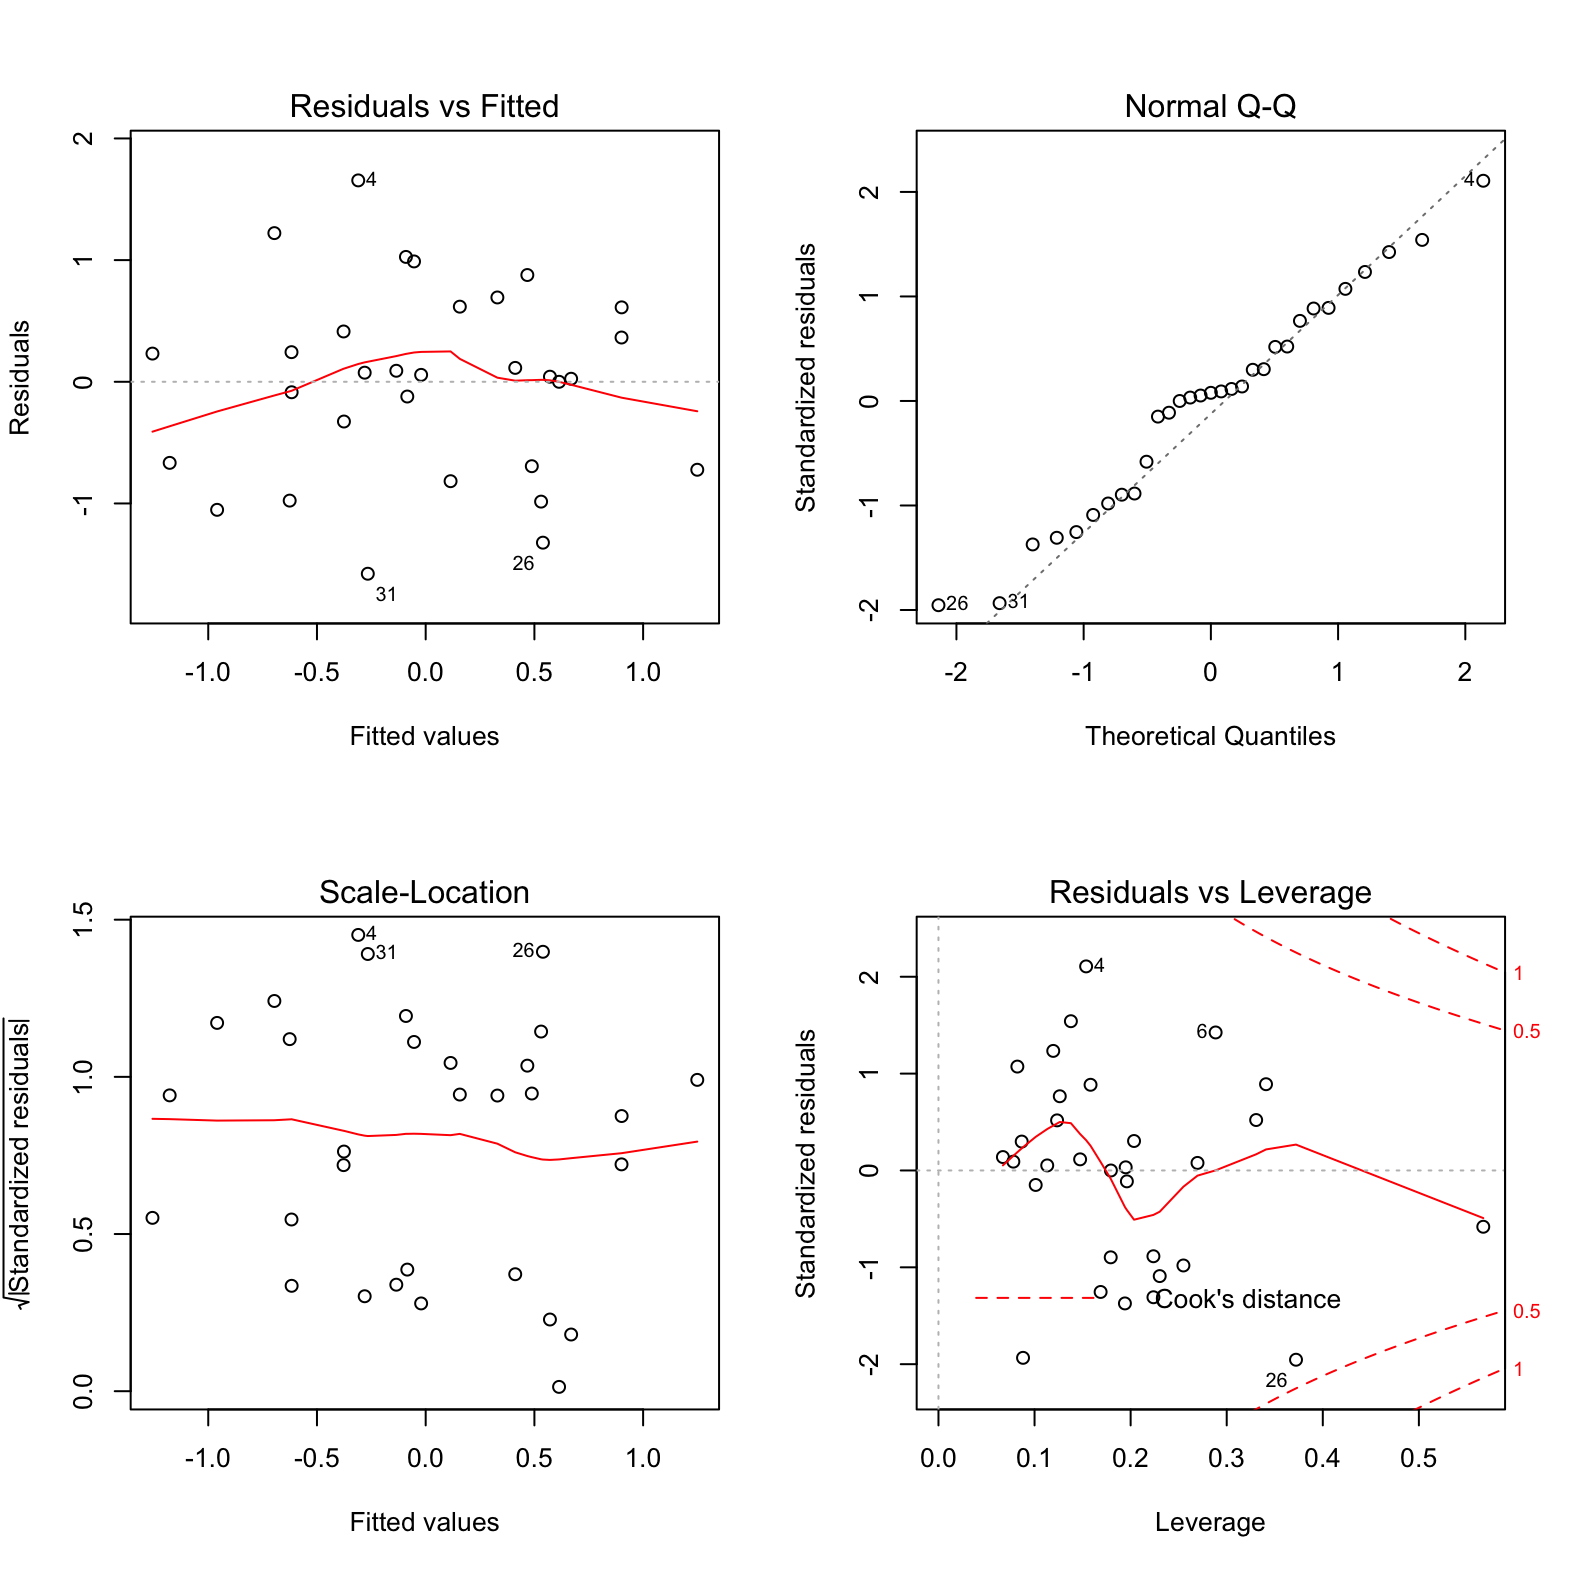
\includegraphics[width=8cm]{regP.png}
		\centering
		\caption{残差分析图}
		\label{fig:17}
	\end{figure}
	由上图可知,残差是正态分布,落在[-2,2]之间,存在极端值第4、31、26个观测对模型有一定影响。
	
	从上图中可以看出,该模型通过F检验后显著性为0.022,在显著性水平为95\%的条件下,模型是显著的,即上述变量中存在可以对球队胜率有影响的变量,模型的R\^2是0.27,说明所选的自变量对球队胜率只可以解释27\%,在本文选择的指标之外,还有73\%的未知因素对球队胜率有影响。每个便利那个的t检验,在95\%显著性下,只有球员利用率和球员效率和球队控球时间对球队胜利概率有显著影响。球员利用率越高,球队胜率越低,球员效率越高,球队胜率越高,球队球员控球时间越长,球队的胜率越低。\\
	
	


	
\item {\bfseries 主成分分析建模:}由于本模型的变量个数较多,且存在一定的相关性,如果分别对每个指标进行分析,往往是孤立的,不能完全利用数据中的信息,且盲目减少指标会损失很多有用的信息,产生错误的结论。在此利用主成分分析,将n维变量映射到k维数据上。PCA的主要思想是将n维特征映射到k维上,这k维是全新的正交特征也被称为主成分,是在原有n维特征的基础上重新构造出来的k维特征。PCA的工作就是从原始的空间中顺序地找一组相互正交的坐标轴,新的坐标轴的选择与数据本身是密切相关的。其中,第一个新坐标轴选择是原始数据中方差最大的方向,第二个新坐标轴选取是与第一个坐标轴正交的平面中使得方差最大的,第三个轴是与第1,2个轴正交的平面中方差最大的。
\\
将上述6个变量进行主成分分析,得到主成分因子的累积贡献率如下:
\begin{table}[h]
	\begin{tabular}{|c|c|c|c|c|c|c|}
		\hline
		\multicolumn{7}{|c|}{ Importance of components:} \\
		\hline
		                        & Comp.1&     Comp.2  &     Comp.3     &  Comp.4    &   Comp.5   &    Comp.6\\
		Standard deviation  &   2.923 &0.337 &0.0742 &2.424e-02&2.227e-02 &1.032835e-02\\
		Proportion of Variance& 0.986&0.013& 0.001& 6.71e-05& 5.726e-05 &1.231e-05\\
		Cumulative Proportion & 0.986& 0.999& 0.99986 &1.00e+00& 1.00e+00 &1.00e+00\\
		\hline
	\end{tabular}
\end{table}
可以看到从第四个主成分开始就已将涵盖了这六个变量的全部信息,我们查看前三个变量的因子载荷矩阵:

 得到第一个主成分$Pc1 =  ORtg\_A    $ ,第二个主成分为$Pc2 = Team\_Poss$, 第三个主成分为$Pc3 = 0.515*Team\_TSR+0.780*Team\_eFGP+0.298 *Team\_USR+0.194*Team\_PER$,说明球队自身的数据涵盖了更多关于球队是否可以获胜的信息,而根据球员数据得到的数据,整体构成了第三个主成分。
 
                      
\begin{table}[h]
	\begin{tabular}{|c|c|c|c|}
		\hline
		\multicolumn{4}{|c|}{Loadings:}\\
		\hline
		Variable	&Comp.1 &Comp.2& Comp.3 \\
		ORtg\_A   &  1.000    & 0& 0\\                              
		Team\_TSR   &   0       & 0&  -0.515\\ 
		Team\_eFGP  & 0&    0&         -0.780 \\
		Team\_USR     &0&0       &    -0.298 \\ 
		Team\_PER  &0&       0&       -0.194\\  
		Team\_Poss     &0&   1.000  &0\\    
		\hline                      
	\end{tabular}
	\centering
	\label{tab:11}
	\caption{主成分因子载荷}
\end{table}

这里做主成分回归,选择三个主成分,采用的最优量化指标为均方根误差RMSEP,得到最终的模型为:

\begin{multline}
  W/L\% = 0.572*ORtg/A+0.110*Team\_TSR+0.0134*Team\_eFGP-0.286*Team\_USR+\\0.228*Team\_PER-0.193*Team\_Poss
\end{multline}




\item {\bfseries 岭回归建模}
最小二乘法的局限性是当变量之间的相关性较强(多重共线性),自变量矩阵不再是满秩矩阵。那就会使得($X^{T}X$)的结果趋近于0,造成拟合参数的数值不稳定性增加(参数间的差距变化很大)。岭回归可以被看作为一种改良后的最小二乘法,它通过向损失中添加L\_{2}正则项(2-范数)有效防止模型出现过拟合,且有助于解决非满秩条件下求逆困难的问题,从而提升模型的解释能力。岭回归的损失函数变为:$L_{loss}=||Y-X'W||^2+\lambda ||W||^2$,得到的参数W的表达式为$W=(X^TX+\lambda I)^{-1}X^TY$
利用岭回归建模得到如下结果:
\begin{table}[h]
	\begin{tabular}{|c|c|c|c|c|c|}
		\hline
		\multicolumn{6}{|c|}{Coefficients:}\\
		\hline
		& Estimate &Scaled estimate& Std. Error (scaled)& t value (scaled) &Pr(>|t|)   \\
		  (Intercept)& -3.287e-15  &            NA   &               NA      &         NA  &     NA  \\
		    `ORtg/A`   &  6.501e-01  &     3.561e+00       &    5.995e-01      &      5.939 &2.87e-09 ***\\
		    Team\_TSR &   -2.988e-02&      -1.636e-01  &         7.226e-01    &        0.226  &  0.821    \\
		    Team\_eFGP &   7.847e-02  &     4.298e-01  &         7.448e-01     &       0.577   & 0.564   \\ 
		    Team\_USR &   -1.477e-01 &     -8.091e-01     &      6.482e-01   &         1.248  &  0.212  \\  
		    Team\_PER   &  1.489e-01&       8.153e-01       &    6.313e-01     &       1.291   & 0.197   \\ 
		    Team\_Poss   &-1.600e-01 &     -8.765e-01   &        5.504e-01   &         1.593 &   0.111   \\ 
		    \hline
		    \multicolumn{6}{|c|}{Signif. codes:  0 ‘***’ 0.001 ‘**’ 0.01 ‘*’ 0.05 ‘.’ 0.1 ‘ ’ 1}\\
		    \hline
		     \multicolumn{6}{|c|}{Ridge parameter: 0.09169586, computed using 4 PCs}\\
		     \hline
		     \multicolumn{6}{|c|}{Degrees of freedom: model 4.812 , variance 4.13 , residual 5.493}\\
		     \hline
	\end{tabular}
\centering
\end{table}
该模型得到结果如上表所示,可以看出只有ORtg/A即进攻效率是显著影响球队胜率的,该模型自动选取岭回归参数0.0917,选取了4个主成分,得到的最终模型为:
\begin{multline}
W/L\% =-3.287e-15+ 0.6501*ORtg/A-0.02988*Team\_TSR+0.07847*Team\_eFGP-\\0.1477*Team\_USR+0.1489*Team\_PER-0.16*Team\_Poss
\end{multline}


\end{enumerate}






  


